\RequirePackage[orthodox]{nag}
\documentclass[11pt]{article}

%% Define the include path
\makeatletter
\providecommand*{\input@path}{}
\g@addto@macro\input@path{{include/}{../../include/}}
\makeatother

\usepackage{../../include/akazachk}

\title{Sustainable Systems Modeling - 114543}
\author{Andres Espinosa}
\begin{document}
\pgfplotsset{compat=1.18}
\maketitle

\tableofcontents

\section{Introduction to System Theory}
\subsection{Context}
A \textbf{system}, denoted as a box with an $S$ inside depicted below in Figure \ref{figure:system}, is a set of entities interacting with each other and with the external environment according to different laws, relationships, and activities.

\begin{figure}[h]
  \centering
    \begin{tikzpicture}[baseline=(S.center)]
    \node[draw, rectangle, minimum width=1cm, minimum height=0.8cm] (S) {$S$};
    \draw[->] ($(S.west)+(-1,0)$) -- node[above] {$u$} (S.west);
    \draw[->] (S.east) -- node[above] {$y$} ($(S.east)+(1,0)$);
    \end{tikzpicture}
  \caption{Abstract system.}
  \label{figure:system}
\end{figure}

A system \textit{reacts} to an external action by an input signal denoted $u$.
The input comes from the outside and impacts the system in some way.
The system then produces an output signal $y$.
Generally, a system's output signal depends on the input signal and a combination of the system's inherent physical and behavioural features.

There is a third set of quantities that characterize the system which represents the full information on the system at an arbitrary moment in time.

\begin{figure}[h]
  \centering
    \begin{tikzpicture}[baseline=(S.center)]
    \node[draw, rectangle, minimum width=1cm, minimum height=0.8cm] (S) {$S$};
    \draw[->] ($(S.west)+(-1,0)$) -- node[above] {$u$} (S.west);
    \draw[->] (S.east) -- node[above] {$y$} ($(S.east)+(1,0)$);
    \draw[<->, red] ($(S.south)+(0,-0.5)$) -- node[right] {$x$} (S.south);
    \end{tikzpicture}
  \caption{Abstract system with a state $x$}
  \label{figure:system_w_state}
\end{figure}

The state vector is denoted $x$.
These values $u,y,x$ are all typically time dependent.
\begin{itemize}
  \item $x(t), u(t), y(t)$
\end{itemize}

\begin{equation}
  \textbf{x}(t) \in X \subseteq \mathbb{R}^n
\end{equation}

\subsection{Introduction to Linear System Theory}
The aim of \textbf{systems theory} is to study the characteristics of cause-and-effect processes involving dynamic systems.
\subsubsection{Vehicle Example of a Dynamic System}
We can consider an example where there is a vehicle with inputs that act on it to output a speed.
Some inputs are control actions, which might represent the gas and brake pedal, and some inputs are exogenous and we have no control to change in the system design but is still an important input such as wind or terrain slope.

\begin{figure}[h]
  \centering
    \begin{tikzpicture}[baseline=(V.center)]
    \node[draw, rectangle, minimum width=2cm, minimum height=3cm] (V) {Vehicle};
    \draw[->] ($(V.west)+(-2,0.5)$) -- node[above] {Wheel} ($(V.west)+(0,0.5)$);
    \draw[->] ($(V.west)+(-2,0)$) -- node[above] {Pedal} ($(V.west)+(0,0)$);
    \draw[->] ($(V.west)+(-2,-0.5)$) -- node[above] {Brake} ($(V.west)+(0,-0.5)$);
    \draw[->] (V.east) -- node[above] {Speed} ($(V.east)+(3,0)$);
    \end{tikzpicture}
  \caption{Vehicle system with multiple inputs and one output.}
  \label{figure:vehicle_system}
\end{figure}

\subsubsection{Models of Dynamic Systems}

The dynamic systems that we are considering are either continuous or discrete in time.
The following describes important notation:
\begin{itemize}
  \item Continous time: $t \in T \subseteq \mathbb{R}$
  \item Discrete time: $ k \in K \subseteq \mathbb{Z}$
  \item Input vector: $ \textbf{u} \in U \subseteq \mathbb{R}^m$
  \item Output vector: $\textbf{y} \in Y \subseteq \mathbb{R}^p$
  \item System state vector: $\textbf{x} \in X \subseteq \mathbb{R}^n$
\end{itemize}

A causal system, any system that depends only on the present and past values of the input for its state, can be modeled as

\begin{equation}
  \textbf{y}(t) = \eta (t_0, t, \textbf{y}(t_0), \textbf{u}[t_0, t])
\end{equation}

where $\eta(\cdot)$ is the input-output relationship and $t_0$ is the initial analysis instant.

A time-invariant system does not depend directly on the timestep $t$, only on the input that has occurred since the initial time.
\begin{equation}
  \textbf{y}(t) = \eta (t_0, \textbf{y}(t_0), \textbf{u}[t_0, t])
\end{equation}

\subsubsection{Water Tank Example}

We can define a very simple Single Input Single Output (SISO) when $m=1, p=1$ shown previously in Figure \ref{figure:system}.

\begin{figure}[htbp]
  \centerline{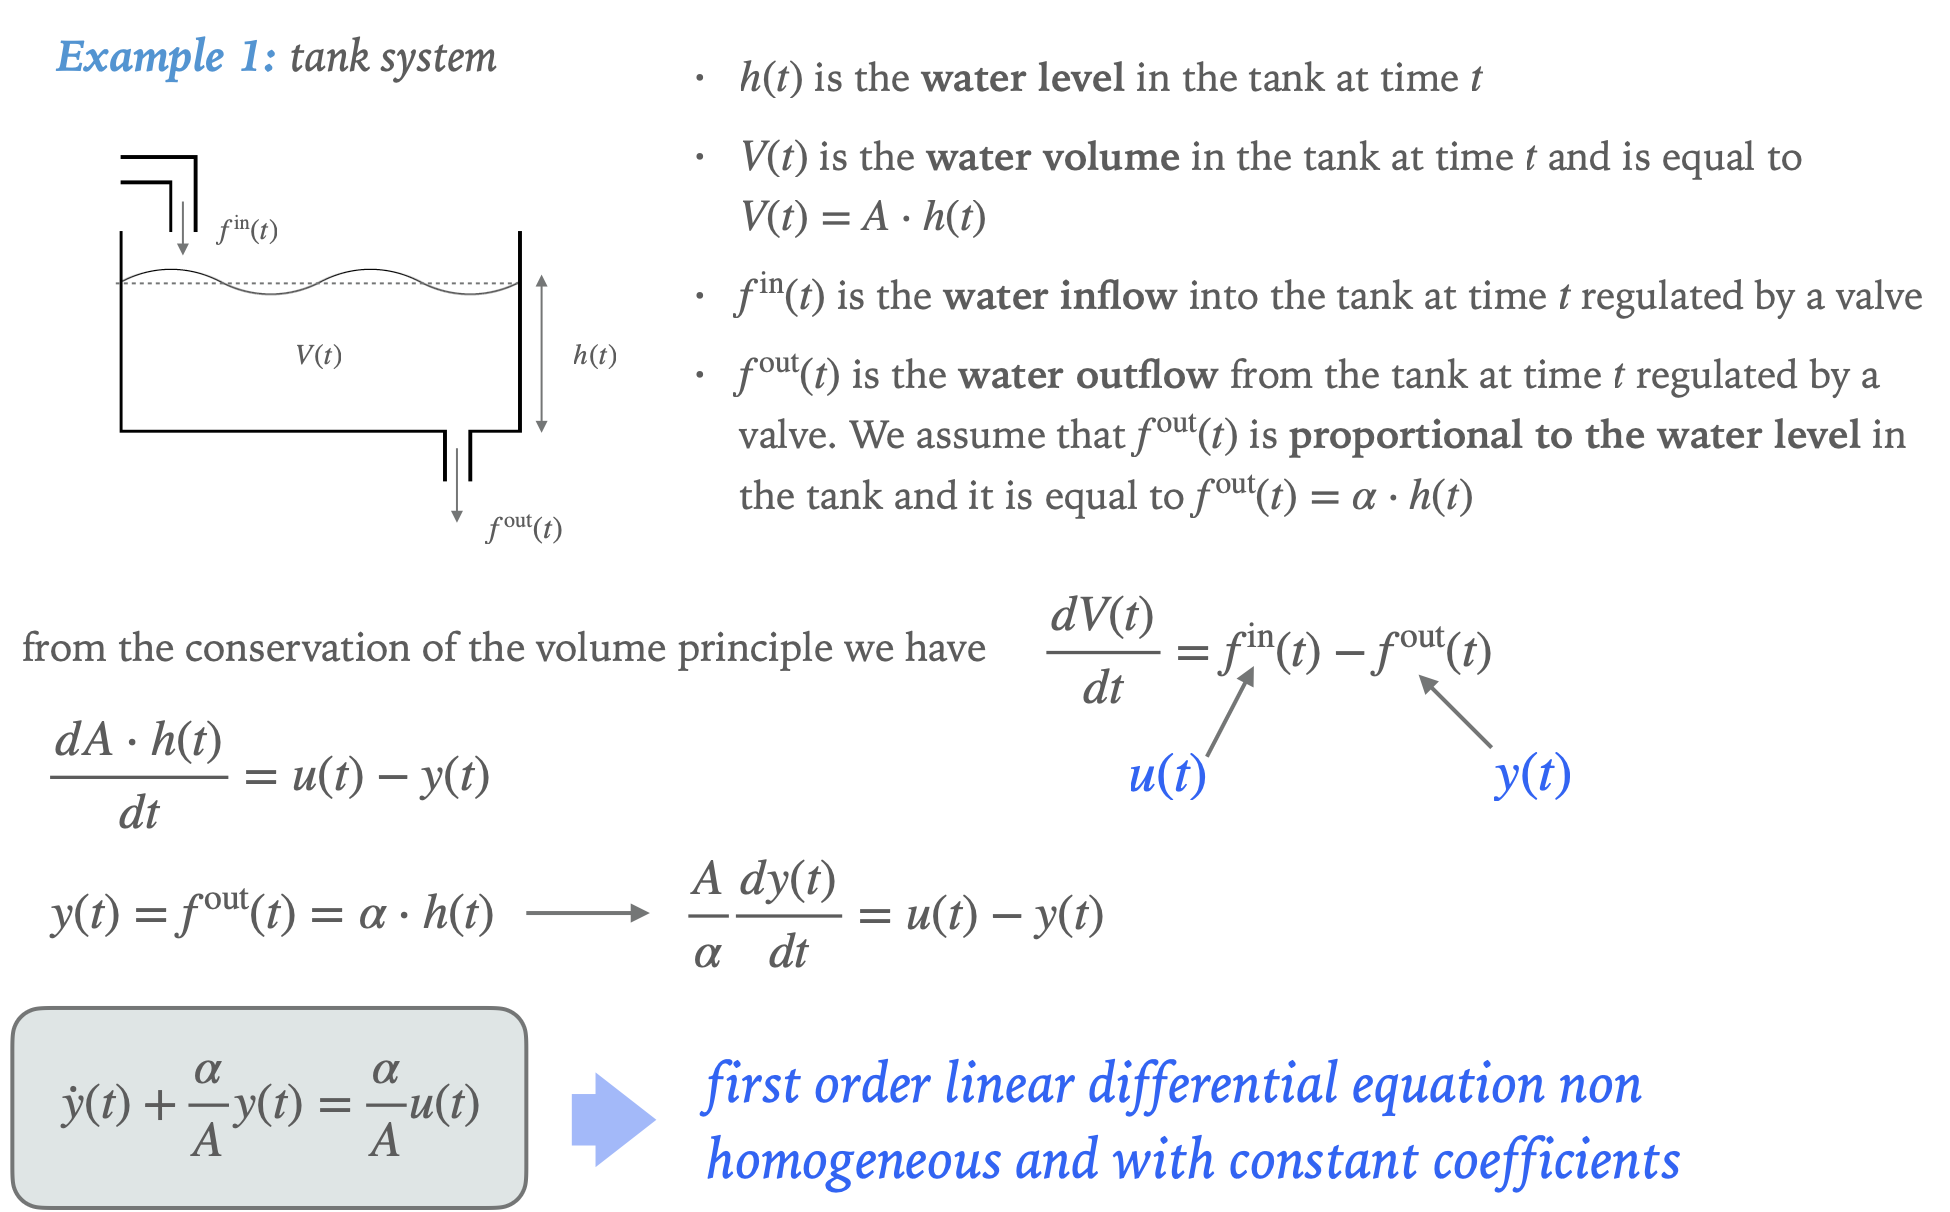
\includegraphics[width=1\textwidth]{../../images/tank_system.png}}
  \caption{A water tank system}
  \label{fig:tank_system}
\end{figure}

In continuous-time LTI systems, the relationship between input and output can always be described by a differential equation of order $n$ with constant coefficients that we need to solve only for $y(t)$.

\subsubsection{Input-Output LTI}
The general equation for an input-output Linear Time-Invariant system is
\begin{equation}
  y^n(t) + a_{n-1}y^(n-1)(t) + \dots + \dots a_1 y^\prime (t) + a_0 y(t) = b_m u^m (t) + b_{m-1} y^(m-1) (t) + \dots + b_1 u^\prime (t) + b_0 u(t)
\end{equation}

or a summed form
\begin{equation}
  \sum_{i=0}^n a_i \frac{d^i y(t)}{d t^i } = \sum_{i=0}^{m} b_i \frac{d^i u(t)}{d  t^i} 
\end{equation}

subject to 
\begin{itemize}
  \item $u,y : T \rightarrow \mathbb{R}$
  \item $n \geq m$
  \item $a_0, \dots, a_n \in \mathbb{R}$ and $a_n=1$
  \item $b_0, \dots, b_m \in \mathbb{R}$
\end{itemize}

In order to solve the linear differential equation and get the response of the system $y(t)$, we need to know the initial conditions of the output at $t=0$ and the applied input over time.
The total response of the system is given by two terms that can be separated output
\begin{equation}
  y(t) = y_n(t) + y_f(t)
\end{equation}

where $y_n(t)$ is the free response of the output that is obtained by having input equal to zero but with a non-zero initial condition and $y_f(t)$ is the forced response of the output which has an initial condition of the output equal to zero.
The free response $y_n(t)$ corresponds to finding the homogenous solution of the differential equation whereas $y_f (t)$ corresponds to finding the particular solution of the differential equations.

\subsubsection{State-Space Representation}
A system can also have more complexity than input-output relationships and may have a collection of parameters and information that are fully indicative of the system called the state.
Below is a digram of the previous vehicle example with the position added to the state as well as the input and output of acceleration and speed.
\begin{figure}[h]
  \centering
    \begin{tikzpicture}[baseline=(V.center)]
    \node[draw, rectangle, minimum width=2cm, minimum height=3cm] (V) {Vehicle};
    \draw[->] ($(V.west)+(-2,0.5)$) -- node[above] {Wheel} ($(V.west)+(0,0.5)$);
    \draw[->] ($(V.west)+(-2,0)$) -- node[above] {Pedal} ($(V.west)+(0,0)$);
    \draw[->] ($(V.west)+(-2,-0.5)$) -- node[above] {Brake} ($(V.west)+(0,-0.5)$);
    \draw[->] (V.east) -- node[above] {Speed} ($(V.east)+(3,0)$);
    \draw[->] (V.south) -- ++(0,-2) node[midway,right] {Position, Speed, Acceleration};
    \end{tikzpicture}
  \caption{Vehicle system with multiple inputs, one output, and state variables.}
  \label{figure:vehicle_system_with_state}
\end{figure}

Now, a causal system can be broken out into two equations
\begin{equation}
\begin{cases}
  \dot(\textbf{x})(t) = \phi(t_0, t, \textbf{x}(t), \textbf{u}(t)) & \text{Transition Function} \\
  \textbf{y}(t) = \eta(t, \textbf{x}(t), \textbf{u}(t)) & \text{Output Transform Function}
\end{cases}
\end{equation}

\begin{figure}[htbp]
  \centerline{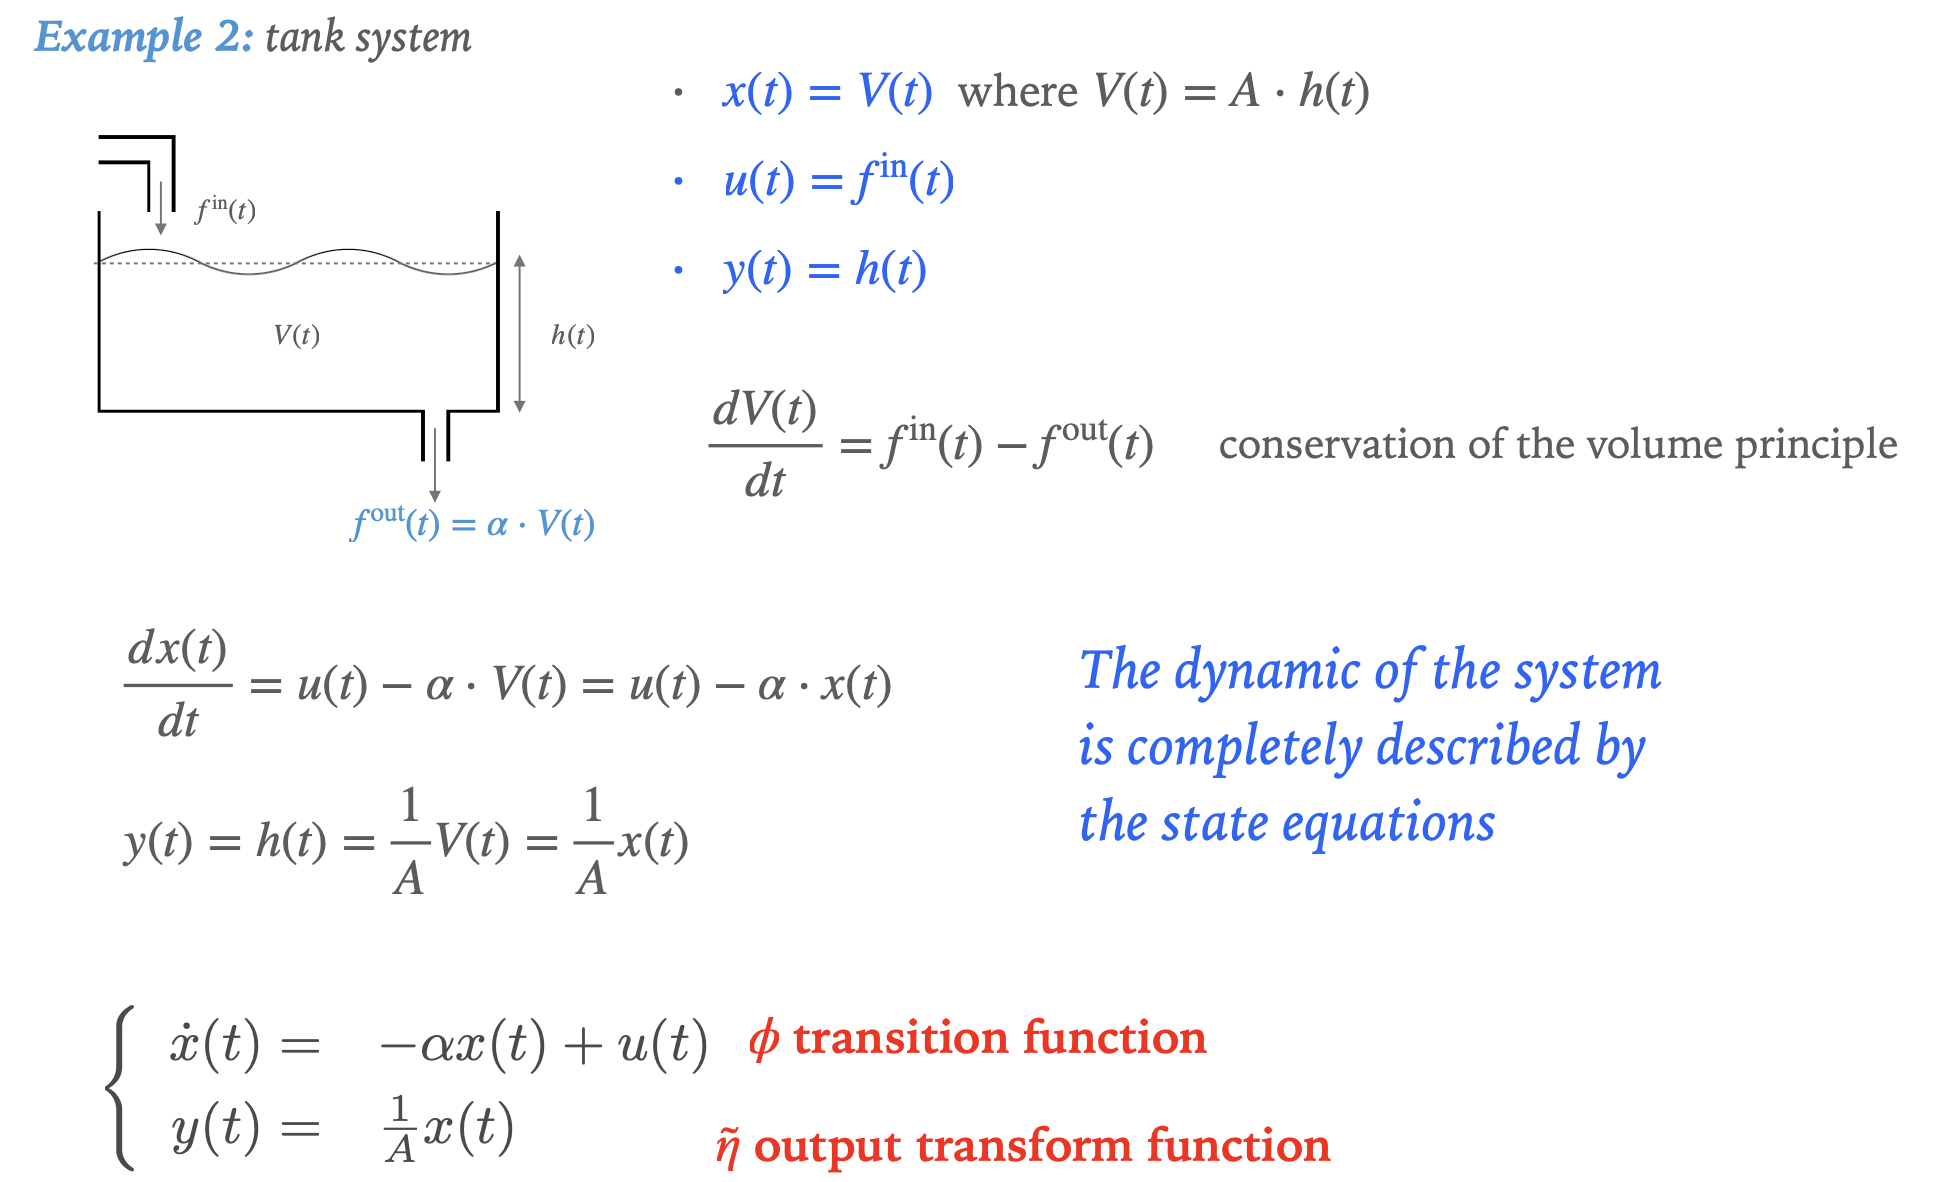
\includegraphics[width=1\textwidth]{../../images/tank_system_state.png}}
  \caption{The water tank example with state}
  \label{fig:tank_system_state}
\end{figure}

In this scenario, the transition function is a differential equation and the output transform function is an algebraic relationship.

\subsubsection{Matrix form State-Space}

We can write the state-space in matrix form for a SISO system
\begin{equation}
  \begin{cases}
    \dot{\textbf{x}}(t) = A \textbf{x}(t) + B u(t) \\
    y(t) = C^T \textbf{x} (t) + D u(t)
  \end{cases}
\end{equation}
where $A \in \mathbb{R}^{n \times n}, B, C \in \mathbb{R}^n, D \in \mathbb{R}$

For example, the following transition and output functions
\begin{equation}
  \begin{cases}
    \dot{x}_1 (t) = x_2 (t) \\
    \dot{x}_2 (t) = -\frac{k}{m} x_1 (t) - \frac{h}{m} x_2 (t) + \frac{1}{m} u(t) \\
    y(t) = x_1 (t)
  \end{cases}
\end{equation}

can be turned into the following set of matrix equations


\begin{align}
  \dot{\textbf{x}} (t) = 
  \begin{bmatrix}
      0 & 1 \\ - \frac{k}{m} & - \frac{h}{m}
  \end{bmatrix}
  \textbf{x} (t)
  +
  \begin{bmatrix}
    0 \\ \frac{1}{m}
  \end{bmatrix}
  u(t)
  , \quad
  y(t) =
  \begin{bmatrix}
    1 \\ 0
  \end{bmatrix}^\top 
  \textbf{x}(t)
\end{align}

\subsubsection{State Total Response}
Similar to the output response, we can break up the system state into the two forced and free terms.

\begin{equation}
  \textbf{x}(t) = \textbf{x}_n + \textbf{x}_f 
\end{equation}

\subsection{Discrete Time}
We can divide timesteps into $k$ intervals and represent a similar input-output relationship as the continuous analogue with the following
\begin{align}
  y(k-n) + a_{n-1} y(k-n+1) + \dots + a_1 y(k-1) + a_0 y(k) \\
  = b_m u(k-m) + b_{m-1} u(k-m + 1) + \dots + b_1 u(k-1) + b_0 u(k)
\end{align}

Our objective is to find the response/output of the system $y(k)$.
We can do this by solving the linear differential equation with constant coefficients.

Similarly to the continuous case, we can divide the total response of a system $y(k)$ into two terms.

\begin{equation}
  y(k) = y_n(k) + y_f(k)
\end{equation}

where $y_n$ is the free response with the input equal to zero and the initial conditions non-zero and $y_f$ is the forced response with initial condition zero.

\subsubsection{Input-Output Representation}
Consider a warehouse with one type of product and $n(k)$ be the number of products in the system.
Every time step $k$ there is a flow $q^{in}(k), q^{out}(k) = h \times n(k) $

\begin{equation}
  n(k+1) = n(k) + q^{in}(k) - hn(k) = (1-h) n(k) + q^{in}(k)
\end{equation}

In this scenario, we have one input $u(k) = q^{in}(k)$ and one output $y(k) = \alpha n(k)$
\begin{equation}
  y(k+1) - (1-h)y(k) = \alpha u (k)
\end{equation}
This is the input-output representation

\subsubsection{State-Space Representation}

\begin{equation}
  \begin{cases}
    \textbf{x}(k + 1) = \textbf{A} \textbf{x} (k) + \textbf{b} u(k) \\
    y(k) = \textbf{c}^\top \textbf{x} (k) + d u(k)
  \end{cases}
\end{equation}

where in a SISO system these are  $\textbf{A} \in \mathbb{R}^{n \times n}, \textbf{b} \in \mathbb{R}^n, \textbf{c} \in \mathbb{R}^n, d \in \mathbb{R}$ constant matrices (since we are time-invariant) that map how the state influences the next time step state and output.
This likely gets more complicated and are turned into full matrices $\textbf{A}, \textbf{B}, \textbf{C}, \textbf{D}$ when we have multiple inputs and outputs.

In a state-space representation for discrete time, similarly we can break out the $\textbf{x}$ state vector in to 
\begin{equation}
  \textbf{x} (k) = \textbf{x}_n (k) + \textbf{x}_f (k)
\end{equation}

Now, tackling the warehouse problem with two types of products $n_1(k), n_2(k)$ with corresponding flows $q_i^{in}, q_i^{out}$

\begin{gather}
  n_1 (k +1) = (1-h_1) n(k) + q_1^{in}(k) \\
  n_2 (k +1) = (1-h_2) n(k) + q_2^{in}(k) 
\end{gather}

We want to predict 
\begin{equation}
  y(k) = \alpha n_1(k) + \beta n_2(k)
\end{equation}

Switching to the right notations w/ state space

\begin{gather}
  x_1 (k +1) = (1-h_1) x_1(k) + u_1(k) \\
  x_2 (k +1) = (1-h_2) x_2(k) + u_2(k) \\ 
  y(k) = \alpha x_1(k) + \beta x_2(k)
\end{gather}

In the matrix notation, 
\begin{align}
  \textbf{A} =
  \begin{bmatrix}
     1 -h_1 & 0 \\ 0 & 1-h_2
  \end{bmatrix},
  \\
  \textbf{B} = 
  \begin{bmatrix}
    1 & 0\\ 0 & 1
  \end{bmatrix}
  \\
  \textbf{c} = 
  \begin{bmatrix}
    \alpha \\ \beta
  \end{bmatrix}^\top
  \\
  d = 0
\end{align}

\subsubsection{General Matrix Form}
We can turn a set of state equations and the output transform function into a general matrix form of arbitrary $n$ inputs and $m$ outputs.
The general matrix form of a state-space representation is
\begin{equation}
  \begin{cases}
    \textbf{x} (k+1) = \textbf{A} \textbf{x} (k) + \textbf{B} \textbf{u} (k) \\
    \textbf{y}(k) = \textbf{C} \textbf{x} (k) + \textbf{D} \textbf{u} (k)
  \end{cases}
\end{equation}

where 
\begin{itemize}
  \item $\textbf{x}(k) \in \mathbb{R}^p$ is the state vector of $p$ state parameters at timestep $k$
  \item $\textbf{y}(k) \in \mathbb{R}^m$ is the output vector of $m$ outputs at timestep $k$
  \item $\textbf{u}(k) \in \mathbb{R}^n$ is the input vector of $n$ inputs at timestep $k$.
  \item $\textbf{A} \in \mathbb{R}^{p \times p}$
  \item $\textbf{B} \in \mathbb{R}^{p \times n}$
  \item $\textbf{C} \in \mathbb{R}^{m \times p}$
  \item $\textbf{D} \in \mathbb{R}^{m \times n}$
\end{itemize}

\subsection{Signals}
There can be continuous (time $t$) and discrete (timestep $k$) signals.
The unit step function (or Heaviside step) is defined as $\textbf{1}(t)$ or with $H(t)$

\subsubsection{Continuous-Time Signals}
\begin{equation}
  \textbf{1}(t) =
  \begin{cases}
    1 & t \geq 0 \\
    0 & t < 0
  \end{cases}
\end{equation}

The causal version of a signal is the version that starts only at $t=0$ and is defined as $f(t) = 0, t <0$.
We can use the \textbf{1}(t) to truncate or translate functions over the time axe as seen in Figure \ref{fig:truncated_signal}

\begin{figure}[htbp]
  \centerline{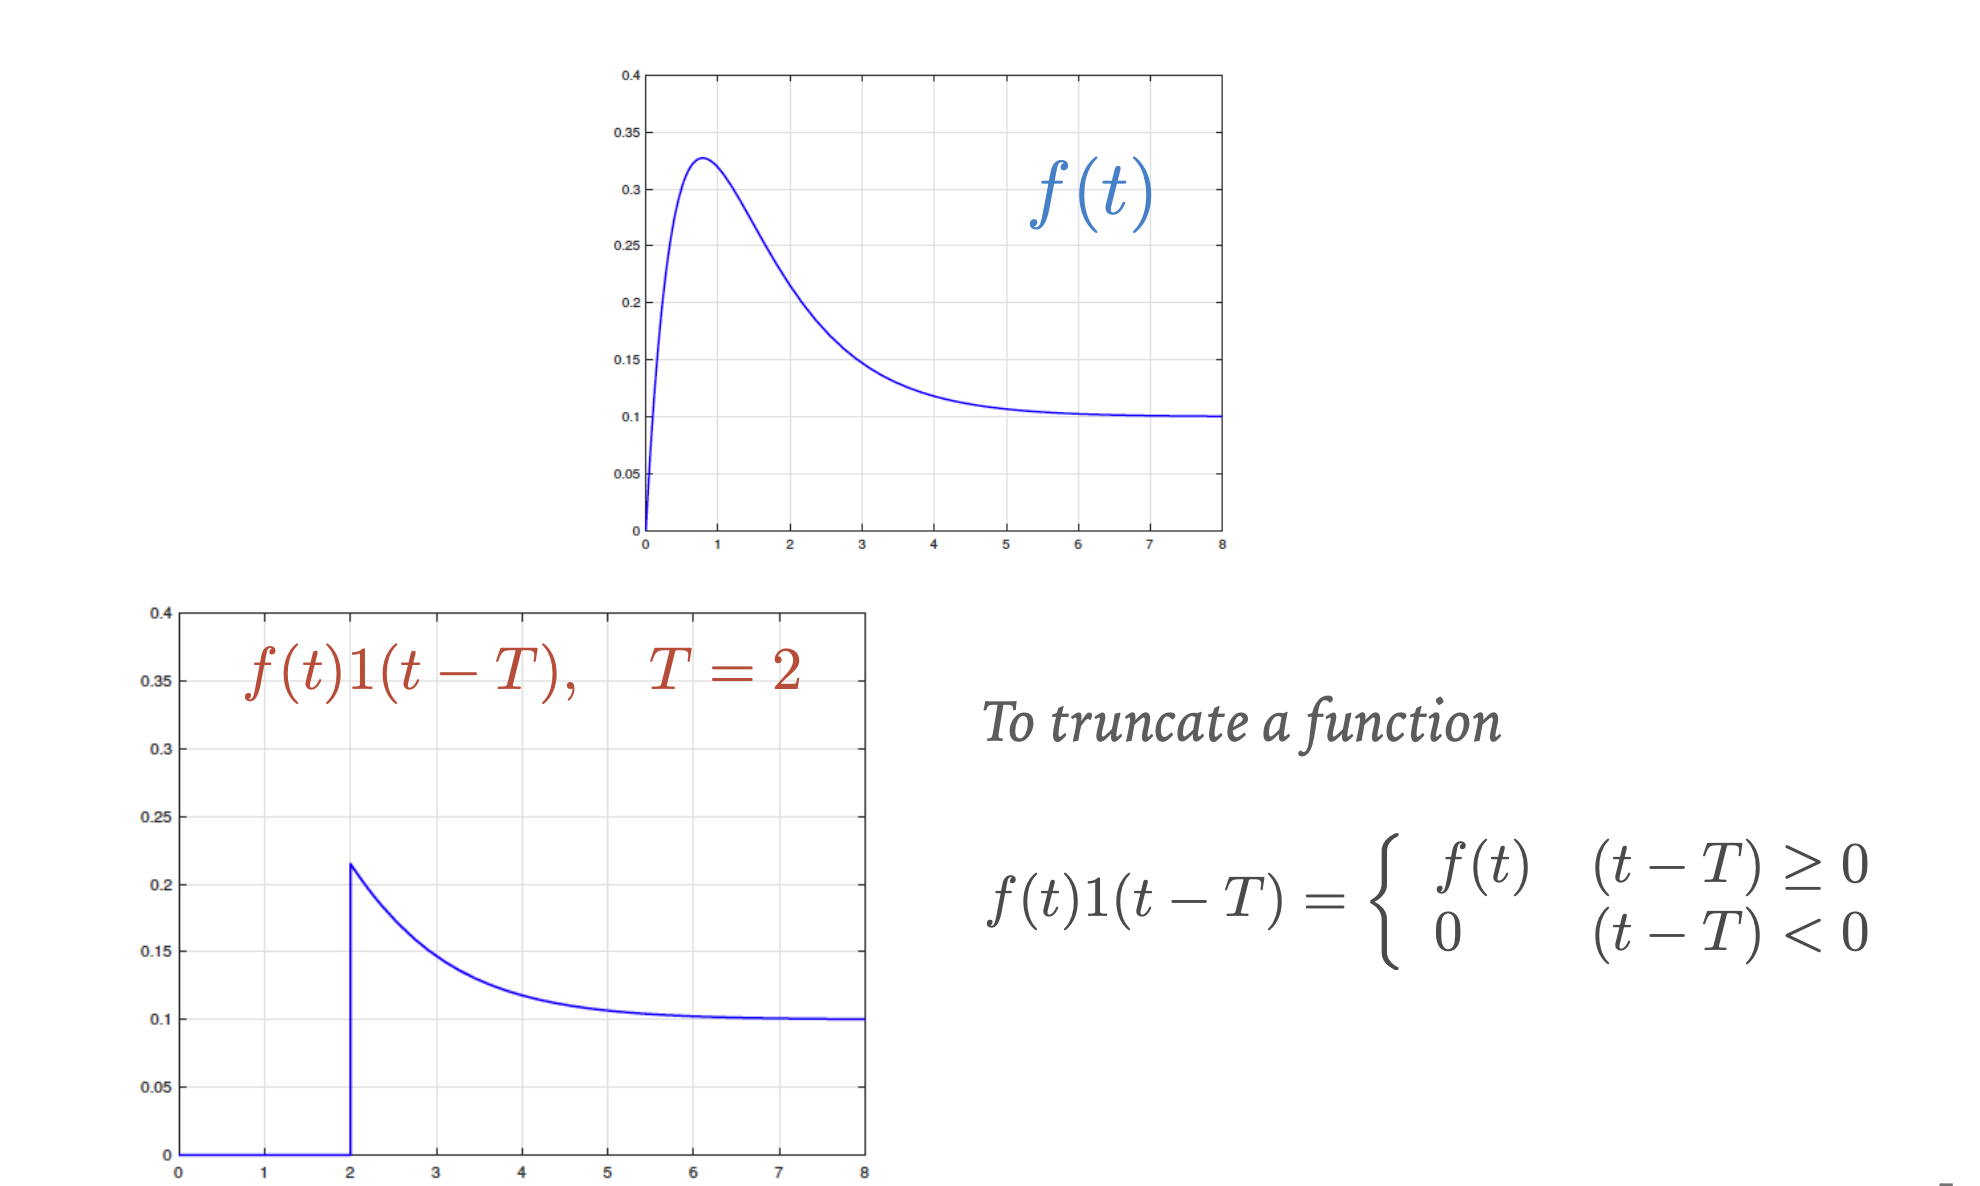
\includegraphics[width=1\textwidth]{../../images/truncated_signal.png}}
  \caption{A signal truncated using the heaviside function}
  \label{fig:truncated_signal}
\end{figure}

Frequently, we can't practically use the unit step function due to its undefined derivative and numerical stability problems.
So, we use a linear variation with $\frac{1}{D}$ as the angular coefficient.
$D$ represents the amount of smoothing we apply to approximate the unit step.
When $D \longrightarrow 0$, the step becomes ideal and its derivative is named Dirac Delta $\delta(t)$

\begin{equation}
  \int_{a}^{b} \delta (t) dt =
  \begin{cases}
    1 & 0 \in (a,b) \\ 
    0 & 0 \notin (a,b)
  \end{cases}
\end{equation}

The main purposes of this dirac delta is to extract the value of a function at zero $f(0)$ or to model the signal with high intensity and low duration as a spike or impulse.

The integral of the unit step function gives us the unit ramp function

\begin{equation}
  \int_{-\infty}^{t} \textbf{1} (\tau) d \tau = t \textbf{1}(t) = r(t)
\end{equation}

\begin{equation}
    r(t) = 
  \begin{cases}
    t & t \geq 0 \\ 0 & t < 0
  \end{cases}
\end{equation}

The exponential signal is also an important signal
\begin{equation}
  f(t) = e^{at} \textbf{1} (t) = 
  \begin{cases}
    e^{at} & t \geq 0 \\
    0 & t < 0
  \end{cases}
\end{equation}

where $a \in \mathbb{R}$

A critical system is a system that goes to infinity.
An affine function or parabolic function is a critical system whereas a harmonic function is not.

Sine and cosine signals are the harmonic functions with amplitude $A \in \mathbb{R}$ and radian frequency $w$.
\begin{gather}
  f(t) = A sin(wt) \textbf{1} (t) \\
  A cos (wt) \textbf{1} (t)
\end{gather}

We can also have sine and cosine signals where the amplitude is actually a function. 

\begin{figure}[htbp]
  \centerline{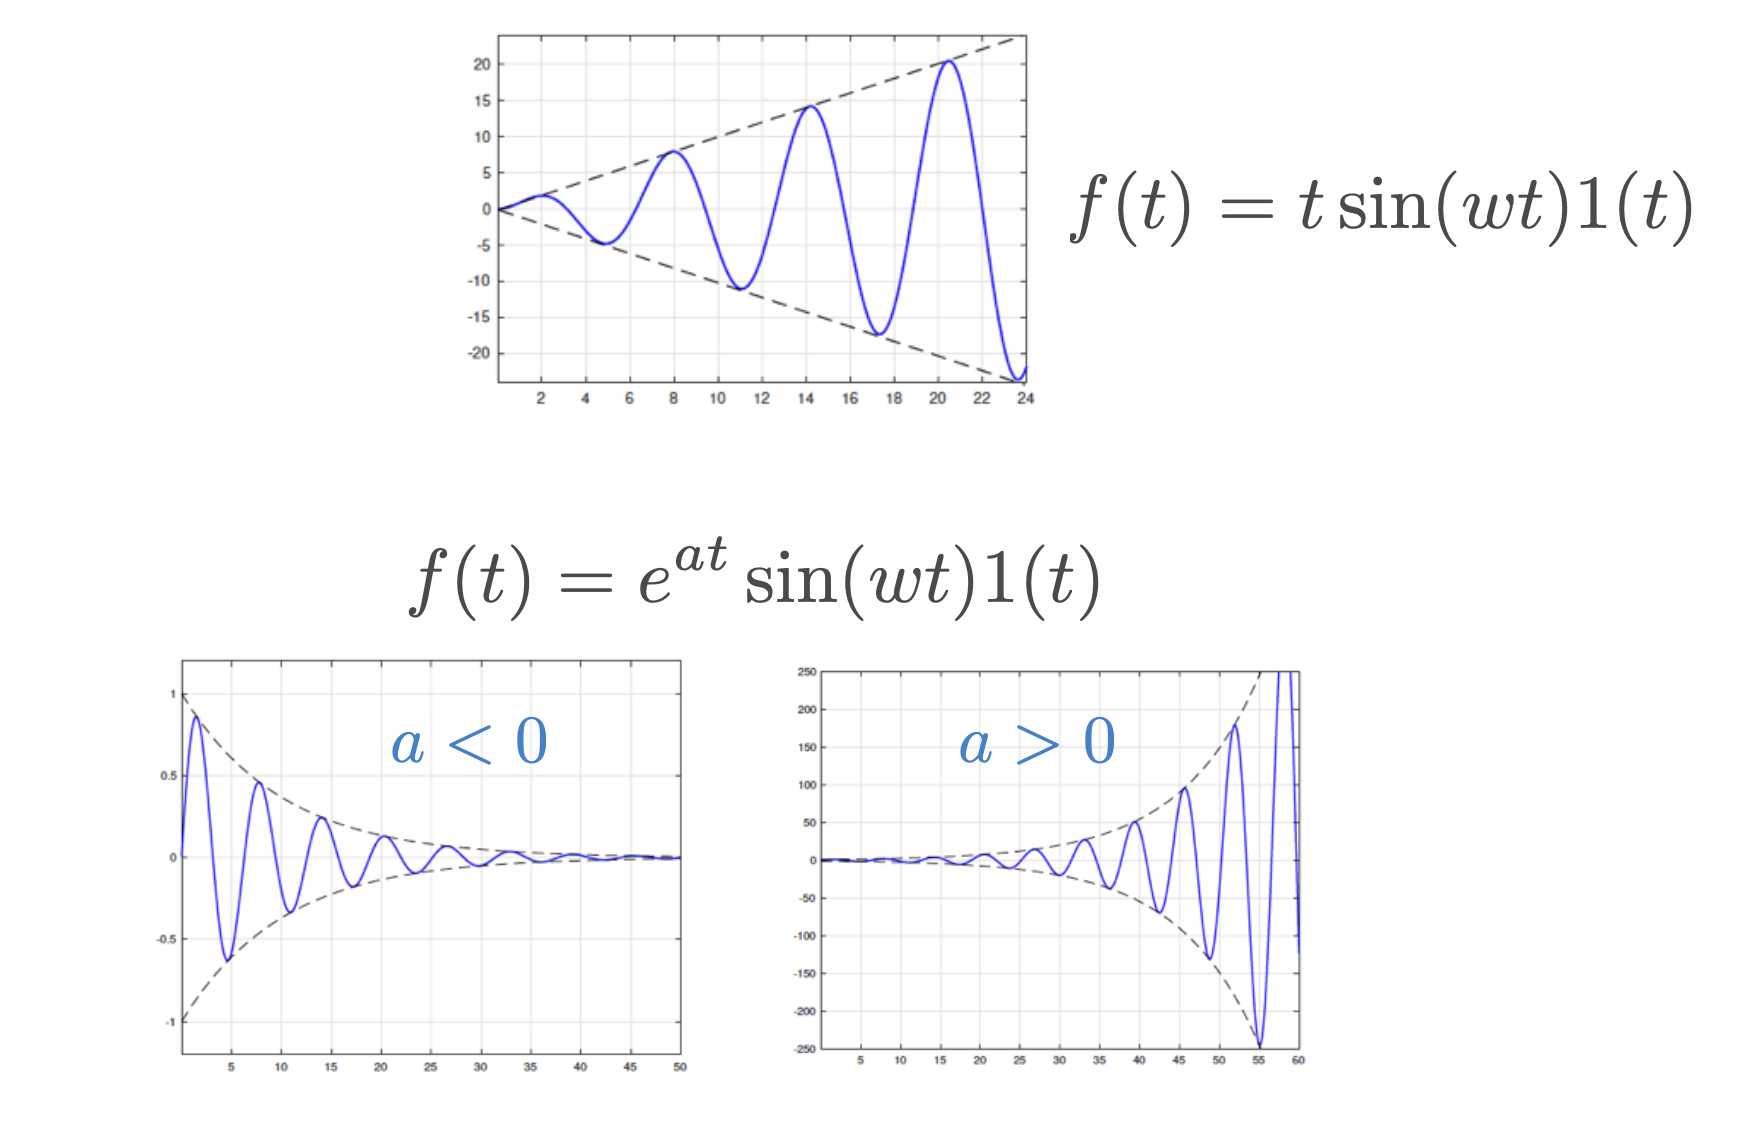
\includegraphics[width=1\textwidth]{../../images/functional_amplitude_harmonic.png}}
  \caption{Sine and cosine functions with functions as amplitude}
  \label{fig:functional_amplitude_harmonic}
\end{figure}

\subsubsection{Discrete-Time Signals}
The same signals present in continuous-time have their analagous discrete-time counterparts using $k$ instead of $t$.

\begin{figure}[htbp]
  \centerline{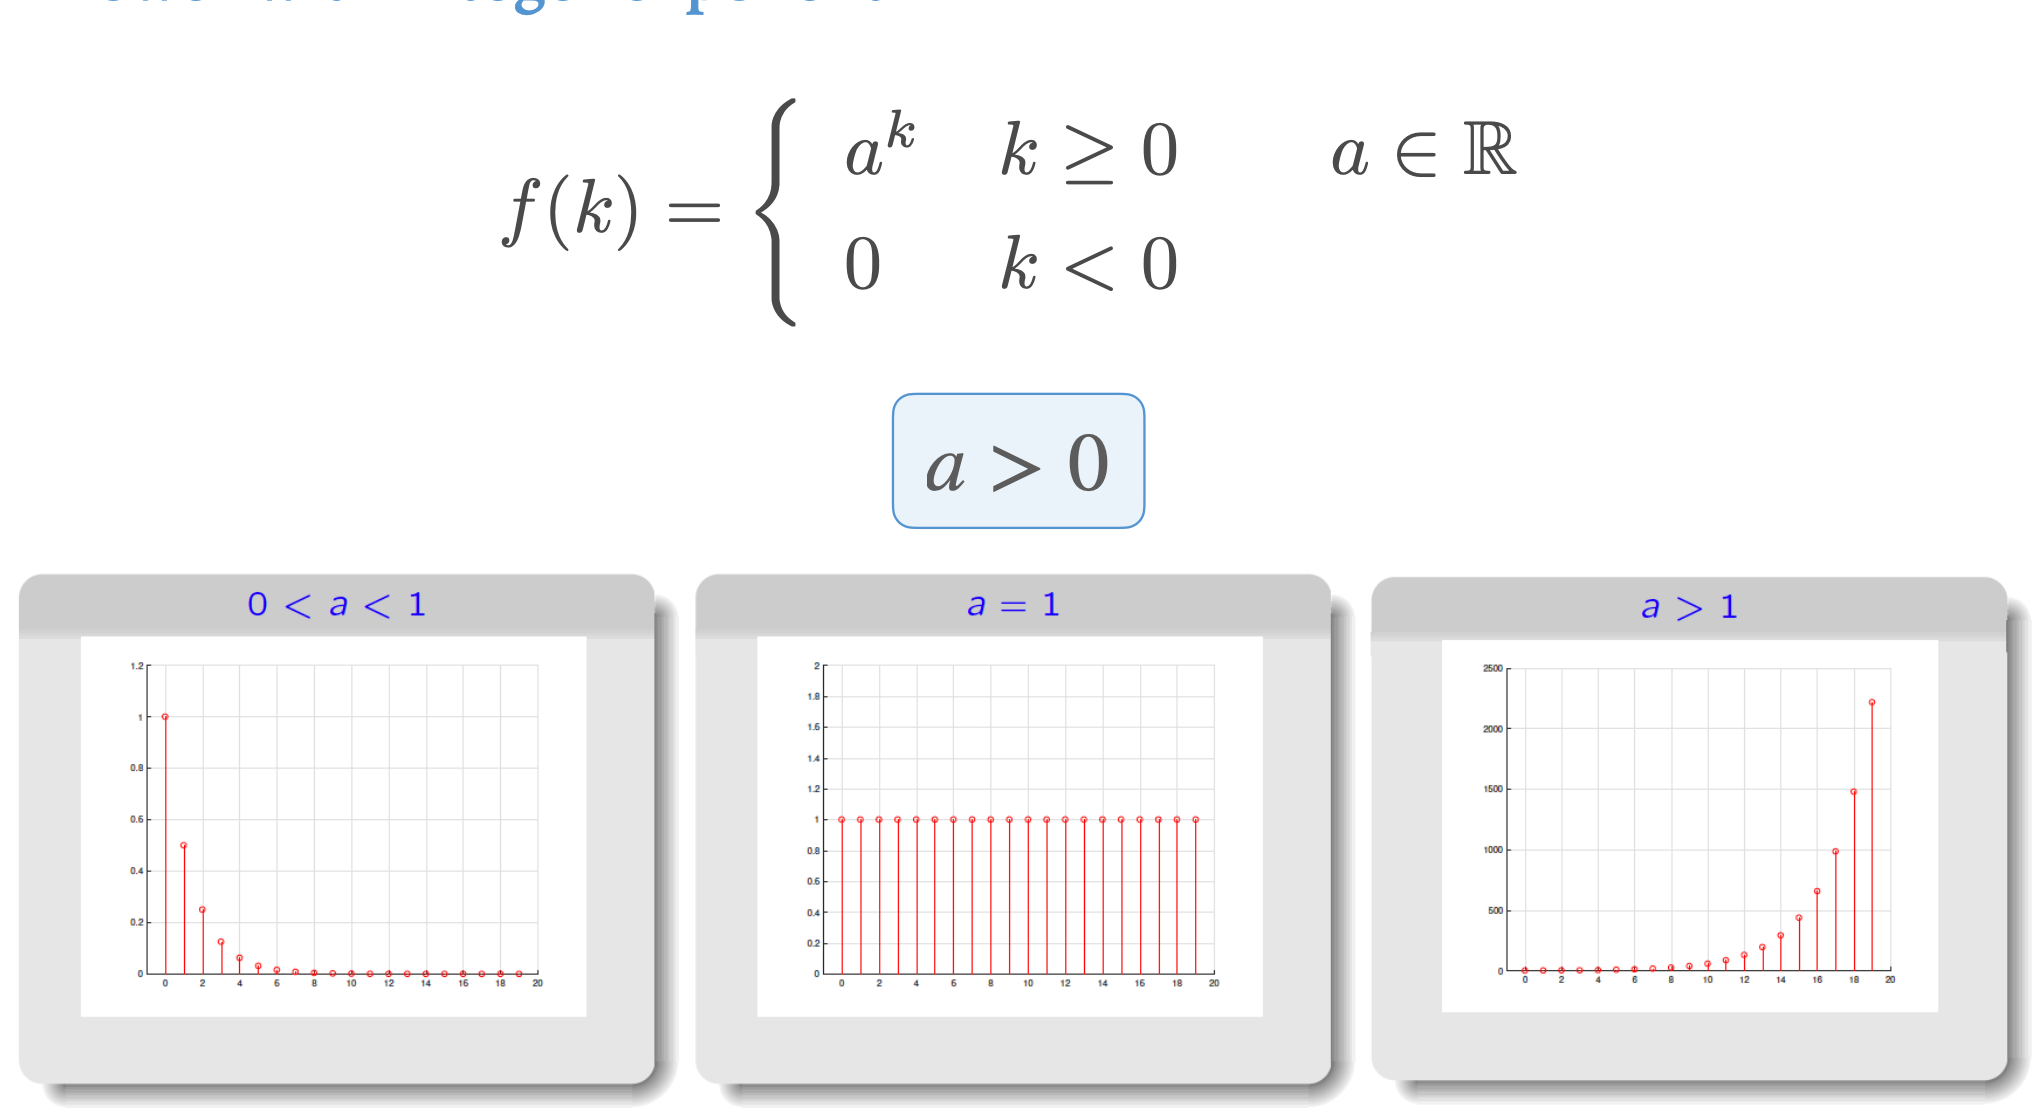
\includegraphics[width=0.75\textwidth]{../../images/discrete_exponential.png}}
  \caption{A discrete exponential signal}
  \label{fig:discrete_exponential}
\end{figure}

\subsection{Laplace}
\subsubsection{Laplace Transform}
The laplace transform is a linear integral operator that converts a function of a real variable (time-domain) to a function of a complex variable (s-domain) $ \mathcal{L}  : f(t) \longrightarrow F(s), \mathcal{L} \{ f(t)\} = F(s), \mathcal{L}^{-1} \{ F(s) \} = f(t)$

\begin{equation}
  \mathcal{L} \{ f(t) \} = \int_{0^{-}}^{\infty} f(t) e^{-st} dt = F(s)
\end{equation}
is called the Laplace transform of $f(t)$ and is indicated as $F(s)$ where $s = a + bj $.

\subsubsection{Laplace Transform Examples}
\textbf{First Example}: $f(t) = 1(t)$

\begin{gather}
  \mathcal{L} \{ 1(t) \}  =  \int_{0^-}^{\infty} 1(t) e^{-st} dt = - \frac{e^{-st}}{s} |_{0^-}^{\infty}= 0 - (-\frac{1}{s}) = \frac{1}{s}
\end{gather}

\textbf{Second Example}: $f(t) = 3e^{-t} + 2t + cos (2t)$
\begin{gather}
  \mathcal{L}\{ 3e^{-t} \} = 3 \frac{1}{s+1} \\
  \mathcal{L}\{ 2t \} = \frac{2}{s^2} \\
  \mathcal{L}\{ cos (2t) \} = \frac{s}{s^2 + 4} \\
  \therefore
  \mathcal{L}\{ f(t) \} = 3 \frac{1}{s+1} + \frac{2}{s^2} + \frac{s}{s^2 + 4}
\end{gather}



\subsubsection{Properties}
\begin{itemize}
  \item Linearity: $\mathcal{L} \{ a f_1(t) + b f_2(t) \} = a \mathcal{L} \{ f_1(t) \} + b \mathcal{L} \{ f_2(t) \} $
  \item Time Shift: $\mathcal{L} \{ f(t-T)1(t-T) \}  = e^{-Ts} \mathcal{L} \{ f(t) \}$
  \item Shifting over complex plane: $\mathcal{L} \{ e^{at} f(t) \} = F(s-a) = \mathcal{L} \{ e^{at} f(t) \}$
  \item Time scaling: $\mathcal{L} \{ f(\frac{t}{a}) \} = a F(as)$ where $a \in \mathbb{R}$
  \item Derivative Laplace transform: $\mathcal{L} \{f^\prime (t)\} = sF(s) - f(0^{-}) $
  \item Multiplication by $t^n$: $\mathcal{L} \{ t^n f(t) \} = (-1)^n \frac{d^n F(s)}{d s^n } $
\end{itemize}

The full general laplace transform of the derivative can be written as 
\begin{equation}
  \mathcal{L} \{ f^{(n)} (t) \} = s^n F(s) - s^{n-1} f(0^-) - \dots - f^{(n-1)} (0^-)
\end{equation}

Multiplying by $s$ in the complex domain is equivalent to taking a deriative in the time domain.
Similarly, dividing by $s$ in the complex domain is equivalent to integrating in the time domain.

\subsubsection{Zeros and Poles}
The zeros of the laplace transform are the values of $s$ for which $F(s) = 0$.
The poles of the laplace transform are the values of $s$ for which $F(s) = \infty$.
Naturally, for a rational function the zeros of the laplace transform are the zeros of the numerator and the poles are the zeros of the denominator
\begin{equation}
  F(s) = \frac{N(s)}{D(s)}
\end{equation}
Considering this rational function $F(s)$, the zeros of $F$ are the roots of $N$, and the poles of $F$ are the roots of $D$.

For example, for the function $\mathcal{L}\{ cos (2t) \} = \frac{s}{s^2+4}$, the zero of the laplace transform is $z_1 = 0$ and the poles are $p_1, p_2 = \pm j2$ with multiplicity $\mu_{1,2} = 1$.
The poles have a correlation with the original function $f(t)$.

The following list correlations with single multiplicity poles:
A positive real-valued pole indicates that the function $f(t)$ increases over time and is a critical signal.
A negative real-valued pole indiciates that the function $f(t)$ decreases over time and converges to 0 over time.
A zero real-valued pole indicates that the function $f(t)$ is horizontally symmetric and does not diverge or converge to 0 over time.

With multiple multiplicity poles, the same is true except for the fact that a zero does not diverge.
With multiple multiplicity poles, the zero real-valued functions are also critical signals.

\subsubsection{Inverse L-Transform}
For an L transform $\mathcal{L}\{ f(t) \} \to F(s)$, we can also define an inverse L-transform that takes a function from the complex space to the real space $\mathcal{L}^{-1}\{ F(s) \} \to f(t)$

One method for the L-inverse transform can take place when the rational function $F(s) = N(s) / D(s)$ has the property of degree of the numerator being strictly lower than the degree of the denominator

\begin{gather}
  F(s) = \frac{N(s)}{D(s)} = \sum_{i=1}^n \frac{A_i}{s-p_i} \\
  = \sum_{i=1}^{r} \sum_{j=1}^{\mu_i} \frac{c_{ij}}{(s-p_i)^j} + \sum_{i=1}^{c} \sum_{j=1}^{\eta_i} \frac{P_{ij} (s)}{((s-\sigma_i)^2 + \omega_i^2)^j}
\end{gather}

In the event that the degree of the numerator is the same as the degree of the denominator, we use a different method for partial fraction expansion.

\begin{gather}
 F(s) = \frac{N(s)}{D(s)} = Q(s) + \frac{N^\prime (s)}{D(s)} \\
 \mathcal{L}^{-1}\{ F(s) \} = q \delta (t) + \mathcal{L}^{-1}\{ \frac{N^\prime (s)}{D(s)} \}
\end{gather}

The initial value theorem is a theorem used to relate complex domain functions to the time domain behavior as time approaches zero.

\textbf{Initial Value Theorem}: 
Given $f(t)$ a function in time-domain and $F(s)$ as the L-transform of $f(t)$ in the complex domain, if the $\lim_{s \to + \infty} sF(s)$ exists, then
\begin{equation}
  \lim_{t\to 0^+} f(t) = \lim_{s \to + \infty} sF(s)
\end{equation}

The final value theorem is used to relate complex domain functions to the time domain as time approaches infinity.

\textbf{Final Value Theorem}:
Given $f(t)$ a function in time-domain and $F(s)$ as the L-transform of $f(t)$ in the complex domain, if the $\lim_{s \to 0^+} sF(s)$ and $\lim_{t \to + \infty} f(t)$ exist, then
\begin{equation}
  \lim_{t\to + \infty} f(t) = \lim_{s \to 0^+} sF(s)
\end{equation}

\subsection{Discrete Transforms}
\subsubsection{Z-Transform}
The z-transform is an operator that transforms a discrete-time signal into the complex domain.
\begin{equation}
  \mathcal{Z}\{ f(k) \} = \sum_{k=0}^{\infty} f(k) z^{-k} = F(z)
\end{equation}
In the expanded form, we have a non-singular component containing the zeros of the function and a singular part where the poles are expressed as negative powers.
\begin{equation}
  \mathcal{Z}\{ f(k) \} = f(0) + \frac{f(1)}{z} + \frac{f(2)}{z^2} + \dots + \frac{f(k)}{z^k}
\end{equation}

The set of values for which $F(z)$ converges is known as the region of convergence (ROC).
For example, for the function $f(k) = 1(k)$, we get 
\begin{equation}
  \mathcal{Z}\{ 1(k) \} = \sum_{k=0}^{\infty} (\frac{1}{z})^k =  \frac{z}{z-1}
\end{equation}
This series converges for $|z|>1$

\subsubsection{Properties}
Similarly to continuous space, there are some properties that hold with z-transforms.
\begin{itemize}
  \item Linearity Property
  \item Shifting over time: Advance)  $\mathcal{Z}\{ f(k+m) \} = z^m [F(z)- \sum_{k=0}^{m-1}f(k)z^{-k}]$, Delay) $\mathcal{Z}\{ f(k-m) \} = z^{-m} F(z)$
  \item Convolution
  \item Scaling: $\mathcal{Z}\{ a^k f(z) \} = F(a^{-1} z)$
  \item Differentiation: $\mathcal{Z}\{ k f(k) \} = -z \frac{d }{d z} F(z) $
\end{itemize}

\subsubsection{Poles}
A main difference between the laplace and Z transforms are the correlation with the poles of the function $f(k)$ and the transform $Z$.
With a function that only has one pole, values inside the unit circle are not critical, and parts outside are.
This is also the case for the functions that have simple complex conjugate poles, where those with poles outside of the unit circle are critical and the others are not.
This is even the case for those with multiple real poles.
\begin{itemize}
  \item If $|a| > 1$, f(k) is divergent
  \item If $|a| < 1$, f(k ) converges to 0
  \item If $|a| = 1$, neither
\end{itemize}

\subsubsection{Inverse Z-Transform}
To perform the z-inverse transform we need to do the partial fraction expansion.

\begin{figure}[htbp]
  \centerline{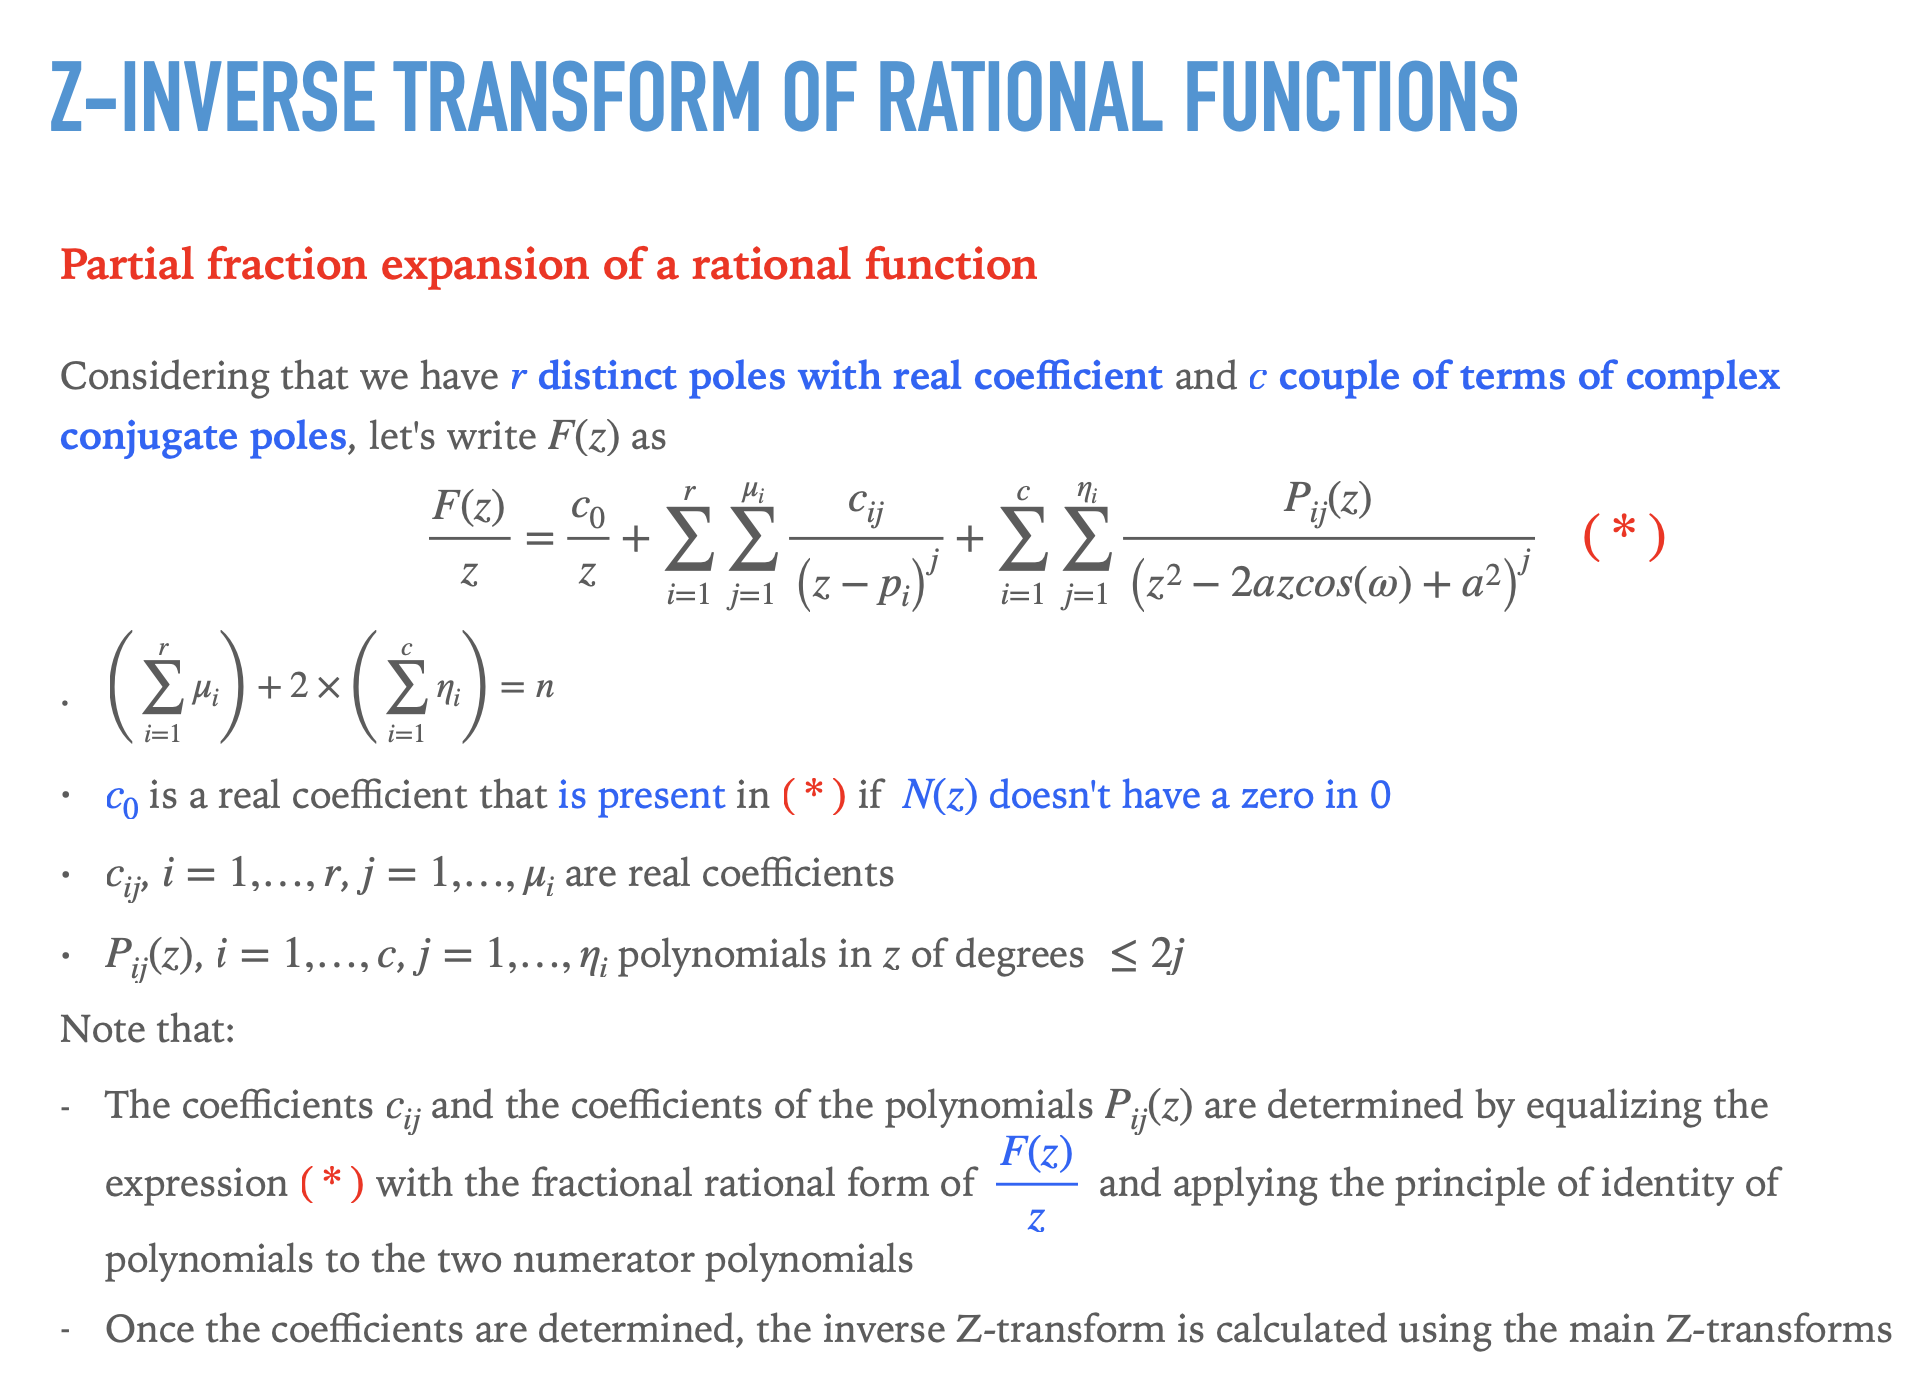
\includegraphics[width=1\textwidth]{../../images/z_inverse_transform.png}}
  \caption{Z-inverse transform}
  \label{fig:z_inverse_transform}
\end{figure}

\begin{gather}
  F(z) = \frac{z}{z^2+z-2} = \frac{z}{(z+2)(z-1)}\\
  \frac{F(z)}{z} = \frac{1}{(z-1)(z+2)} = \frac{c_{11}}{z-1} + \frac{c_{21}}{z+2} \\
  c_{11}(z+2) + c_{21}(z-1) = 1 \\
  c_{21}(-2-1) = 1, c_{11}(1 + 2) = 1 \\
  c_{21} = -\frac{1}{3}, c_{11} = \frac{1}{3} \\
  \text{plug back in: } F(z) = \frac{1}{3}\frac{z}{z-1} - \frac{1}{3} \frac{z}{z+2}
\end{gather}

\textbf{Initial value Theorem}:
\\ 
\framebox[\linewidth]{
    \begin{minipage}{\dimexpr\linewidth-2\fboxsep-2\fboxrule\relax}
        \textbf{Theorem: } 
        given $f(k)$ a DT-signal and $F(z)$ the Z-transform of $f(k)$, if the $\lim_{z \to \infty}$ exists, then
        \begin{equation}
          f(0) = \lim_{z \to \infty} F(z)
        \end{equation}
    \end{minipage}
}

\textbf{Final value Theorem}:
\\
\framebox[\linewidth]{
    \begin{minipage}{\dimexpr\linewidth-2\fboxsep-2\fboxrule\relax}
        \textbf{Theorem: }
        given $f(k)$ a DT-signal and $F(z)$ the Z-transform of $f(k)$, if the limits below exist, then
        \begin{equation}
          \lim_{k \to \infty} f(k) = \lim_{z \to 1} (1-z^{-1}) F(z)
        \end{equation}
    \end{minipage}
}

\subsection{Solutions of a System}
\subsubsection{Input-Output}
The input-output representation of a continuous time LTI system consists of the differential equation:
\begin{equation}
  y^{(n)} (t) + a_{n-1} y^{n-1}(t) + \dots + a_1 y^{(1)}(t) + a_0 y(t) = b_m u^{(m)} + \dots + b_0 u(t)
\end{equation}
we can solve the input of the input-output representation using the laplace transform.
We use the laplace transform of the derivative function to expand it and turn it into the complex domain for both the left side and the right side.
We can also rearrange it to get the following laplace transformed version:
\begin{gather}
  s^n Y(s) + a_{n-1} s^{n-1} Y(s) + \dots + a_0 Y(s) - I(s,y(0^{-}), \dots, y^{n-1}(0^-)) \\ =
  b_m s^m U(s) + b_{m-1} s^{m-1} U(s) + \dots + b_0 U(s)
\end{gather}
where $I$ is a polynomial in $s$ whose coefficients are a function of the initial conditions of the output.

We can rearrange this for the current state $Y(s)$ as

\begin{gather}
  Y(s) = \frac{I(s,y(0^-), \dots, y^{(n-1)}(0^-))}{s^n + a_{n-1} s^{n-1} + \dots a_1s + a_0} + \frac{b_m s^m + b_{m-1} s^{m-1} + \dots + b_0}{s^n + a_{n-1} s^{n-1} + \dots + a_1s + a_0} U(s)
\end{gather}

These two fractions can also be split into the free and forced response of the output.
\begin{gather}
  Y_n(s) = \frac{I(s,y(0^-), \dots, y^{(n-1)}(0^-))}{s^n + a_{n-1} s^{n-1} + \dots a_1s + a_0} \\
  Y_f(s) = \frac{b_m s^m + b_{m-1} s^{m-1} + \dots + b_0}{s^n + a_{n-1} s^{n-1} + \dots + a_1s + a_0} U(s)
\end{gather}

\subsubsection{Transfer Function}
The forced response of the system can be written as 
\begin{equation}
  Y_f(s) = T(s) U(s)
\end{equation}

\begin{equation}
  T(s) = \frac{b_m s^m + b_{m-1} s^{m-1} + \dots + b_0}{s^n + a_{n-1} s^{n-1} + \dots + a_1s + a_0} 
\end{equation}
The roots of the numerator of the transfer function are the zeros of the system and the those of the denominator are the poles of the system.

\subsubsection{State-Space}
\begin{equation}
  \begin{cases}
    \dot{\textbf{x}} (t) = \textbf{A} \textbf{x} (t) + \textbf{B} \textbf{u} (t) \\
    \textbf{y}(t)  = \textbf{C} \textbf{x} (t) + \textbf{D} \textbf{u} (t)
  \end{cases}
\end{equation}

Similarly to the input-output form, this can be solved with lagrange equations nad split up into the forced and natural response of botht he state and the output.
\begin{gather}
  \textbf{x}_n (t) = e^{A(t-t_0)} \textbf{x} (t_0) \\
  \textbf{x}_f (t) = \int_{t_0}^{t} e^{A(t-\tau)} B u(\tau) d\tau \\
  y_n(t) = C e^{A(t-t_0)} \textbf{x} (t_0) \\
  y_f(t) = \int_{t_0}^{t} e^{A(t-\tau)} B u(\tau) d\tau + Du(t)
\end{gather}

We can transform these with laplace so we do not have to raise $e$ to the power of the matrix $A$.

\begin{equation}
  \begin{cases}
    sX(s) - \textbf{x} (t_0^-) = AX(s) + BU(s) \\
    Y(s) = CX(s) + DU(s)
  \end{cases}
\end{equation}

so we finally get the following
\begin{equation}
  \begin{cases}
    X(s) = (s I - A)^{-1} \textbf{x}(t_0^-) + (s I - A)^{-1} BU(s) \\
    Y(s) = C (s I - A)^{-1} \textbf{x}(t_0^-) + [C(s I - A)^{-1}B + D] U(s)
  \end{cases}
\end{equation}

\subsubsection{Example 4 State Space}
Find $(s I - A)^{-1}$, characteristic polynomial and minimal polynomial of the matrix
\begin{align}
  A =
  \begin{bmatrix}
     -1 & 0 & 0 \\ 
     0 & -1 & 1 \\
     0 & 0 & -2
  \end{bmatrix}
\end{align}

\begin{align}
  (s I - A)^{-1} =
  \begin{bmatrix}
    s +1 & 0 & 0 \\
    0 & s + 1 & 1 \\ 
    0 & 0 & s + 2
  \end{bmatrix}^{-1}
\end{align}

\begin{align}
  |s I - A| = 
    (s+1)^2(s+2)
\end{align}

\subsection{Stability}
\subsubsection{Definition of Stability}
Stability is the property of a system to respond to perturbations by returning to the condition that existed before the perturbation, or at least by not moving away from it indefinitely.
The Lyapunov definition of stability is:
\begin{itemize}
  \item The perturbation is applied to the initial condition of the state
  \item Small perturbations of the initial state produce small perturbations of the state response that may become zero over the long period.
\end{itemize}
\subsubsection{Equilibrium}
Stability is strictly related to the definition of the equilibrium points.

For a generic dynamic LTI system, the equilibrium point is the pair $(\bar{\textbf{x}}, \bar{\textbf{u}})$
and is defined as a point for which the system is subjected to constant input vector $\textbf{u}$ and reaches equilibrium state $\textbf{x}$ in which it remains indefinitely.
In other words, the equilibrium point is such that it nullifies the dynamic of the system.
\begin{equation}
  A \bar{\textbf{x}} + B \bar{\textbf{u}} = 0
\end{equation}

An equilibrium point  $(\bar{\textbf{x}}, \bar{\textbf{u}})$ is said to be Lyapunov stable if for any $\epsilon$ greater than zero, there exists a delta greater than zero.

\begin{equation}
  \| \textbf{x}(0^-) - \bar{\textbf{x}} \| \leq \delta \implies \| \textbf{x}(t) - \bar{\textbf{x}} \| \leq \epsilon \quad \forall t > 0
\end{equation}
This basically means, that for any perturbation from the center point, there will be a limit on how far the system reacts over any time.

An equilibrium point  $(\bar{\textbf{x}}, \bar{\textbf{u}})$ is said to be asymptotically stable if it is Lyapunov stable and there exists a delta greater than zero where
\begin{equation}
  \| \textbf{x}(0^-) - \bar{\textbf{x}} \| \leq \delta \text{ and } \lim_{t \to \infty} \| \textbf{x}(t) - \bar{\textbf{x}} \| = 0
\end{equation} 

Effectively, Lyapunov stable means that disturbing the point from the equilibrium point will cause it to not spiral and diverge.
Asymptotically stable means that disturbing the point from the equilibrium will cause it to return to the equilibrium point.

An equilibrium point is said to be unstable if it is not Lyapunov stable.

\subsubsection{System Stability}
Stability is a property of the system and relies on $A$ the matrix that characterizes the system and does not respond on any specific parts of the actual equilibrium point.
\begin{equation}
  \delta \dot{\textbf{x}} (t) = A \delta \textbf{x}(t)
\end{equation}

This leads to the following theorem

\framebox[\linewidth]{
    \begin{minipage}{\dimexpr\linewidth-2\fboxsep-2\fboxrule\relax}
        \textbf{Theorem}: a continuous-time LTI system is asymptotically stable if and only if all eigenvalues of the matrix $A$ have negative real part.
    \end{minipage}
}
In other words, the roots of the characteristic polynomial must be negative.
If there is any eigenvalue with a positive real part, then the system is unstable.
If the multiplicity in the minimal polynomial is equal to one for a zero, then that means the algebraic multiplicty is equal to the geometric multiplicity in the characteristic polynomial.


\subsubsection{BIBO}
Bounded Input Bounded Output (BIBO) stability is the system property that any bounded input yields a bounded output

\framebox[\linewidth]{
    \begin{minipage}{\dimexpr\linewidth-2\fboxsep-2\fboxrule\relax}
        \textbf{theorem:} A continuous-time LTI system is said to be BIBO stable if posed $x(0^-) = 0$ and considering $\| u(t) \| \leq M$ with $M \in \mathbb{R}^+$, then there exists an $N$ where 
        \begin{equation}
          \| y(k) \| \leq N
        \end{equation}
    \end{minipage}
}
This property should hold for any limited input over any time.
\begin{equation}
  Y_f(s) = \frac{N_T(s)}{D_T(s)} \frac{N_U(s)}{D_U(s)}
\end{equation}
By deconstructing the input-output with the transfer function into the above, we can see that in order for $Y_f(s)$ to be limited, the denominator of the transfer function $D_T(s)$ must have only negative real part roots.

\framebox[\linewidth]{
    \begin{minipage}{\dimexpr\linewidth-2\fboxsep-2\fboxrule\relax}
        \textbf{Theorem:} A continuous-time LTI system is BIBO stable iff all the roots of the denominator of $T(s)$ have a negative real part.
    \end{minipage}
}
Additionally, any continuous-time LTI system that is asymptotically stable is also BIBO stable.

\subsubsection{Discrete-Time Stability}
For a discrete-time LTI system, the equilibrium points satisfy the relationship
\begin{equation}
  x(k+1) - x(k) = 0 \implies \bar{x}(k) = A\bar{x}(k) + Bu(k)
\end{equation}
The discrete time has analagous definitions for lyapunov stabl, asymptotically stable, and unstable.

\framebox[\linewidth]{
    \begin{minipage}{\dimexpr\linewidth-2\fboxsep-2\fboxrule\relax}
        \textbf{Theorem: } A discrete-time LTI system is asymptotically stable iff all eigenvalues of the matrix $A$ have absolute value lower than one.
    \end{minipage}
}
\subsubsection{Example}
\begin{align}
  x(k+1) =
  \begin{bmatrix}
     1/3 & 0 & 1 \\
     0 & -1 & a \\
     0 & 0 & -1
  \end{bmatrix}
  x(k) + 
  \begin{bmatrix}
    -1 \\ 0 \\ 1
  \end{bmatrix}
  u(k)
  \\
  y(k) = 
  \begin{bmatrix}
    1 \\ -1 \\ 1
  \end{bmatrix}^\top 
  x(k)
  \\
  (zI - A) = 
  \begin{bmatrix}
    z-1/3 & 0 & -1 \\
    0 & z + 1 & a \\
    0 & 0 & z + 1
  \end{bmatrix}
  \\
  \det (zI-A) = 
  (z-1/3)(z+1)^2
\end{align}
\begin{gather}
  \lambda_1 = 1/3, \mu_1 = 1 \\
  \lambda_2 = -1, \mu_2 = 2
\end{gather}
The system is either lyapunov stable or unstable, we will need to find the minimal polynomial and see if the multiplicity is 1 in that or find the geometric multiplicity.
\begin{equation}
  \nu_2 = 3 - rank(A + I)
\end{equation}

\begin{align}
  A + I = 
  \begin{bmatrix}
     4/3 & 0 & 1 \\
     0 & 0 & a \\
     0 & 0 & 0
  \end{bmatrix}
\end{align}

$\nu_2$ is equal to the algebraic multiplicity $2$ when $a=0$, otherwise if $a \neq 0$, the system is unstable.

\subsection{Structure of LTI Systems}
\subsubsection{Structural Properties}
\begin{itemize}
  \item Reachability and Controllability: properties concerning the possibility of driving the state to assume a fixed value by acting on the input
  \item Observability and Constructibility: properties concerning the possibility of determining the initial value of the state from the knowledge of its output
\end{itemize}

\subsubsection{Reachability and Controllability}
\begin{itemize}
  \item A state $\textbf{x}$ is reachable if, considering a finite time interval of any duration, there exists an input function $u(t)$ capable of transferring the state of the system from the zero state to the state $\textbf{x}$.
  \item A state $\textbf{x}$ is controllable if, considering a finite time interval of any duration, there exists an input functioncapable of transferring the state of the system from the state $\textbf{x}$ to the state zero.
\end{itemize}

A system is said to be fully reachable or controllable if every state $\textbf{x} \in \mathbb{R}^n$ is reachable or controllable.
We can also therefore have certain subspaces of states containing the set of reachable and controllable states for a system.
In discrete-time systems, reachability implies controllability but the converse is only truly when $A$ is invertible.

\subsubsection{Observability and Constructibility}
\begin{itemize}
  \item A state $\textbf{x}$ is observable if knowledge of the system allows $x(0^-)$ to be traced.
  \item A state $\textbf{x}$ is constructible if knowledge of the system allows $x(t)$ to be traced.
\end{itemize}


\end{document}
